\section{Feasibility Study with Human Smokers}
\label{sec:feasibility}
The deployed MIBot system was used in a \margindex{Feasibility Study}feasibility study with human smokers. The goal of the study was to determine the impact of a single-session interaction with MIBot and assess its safety for delivery to ambivalent smokers in a real-world setting.

\subsection{Ethics Approval and Consent}
The protocol was approved by the \margindex[Feasibility Study]{ethics approval}University of Toronto Research Ethics Board under protocol number 49997 (approved August~3, 2024) and adhered to all institutional guidelines. Before participating in the study, prospective participants reviewed an online consent form that outlined study aims, procedures, compensation, potential risks, and data handling practices. Participation required explicit electronic consent. Risks were described as minimal but included the possibility that discussing smoking could cause stress or temporarily increase cravings. No personally identifying information was collected, and all data were de-identified prior to release.

\subsection{Participant Recruitment}
\label{sec:recruitment}
\margindex[Feasibility Study]{participant recruitment}[Recruitment]Participants were recruited via \margindex[Feasibility Study, Recruitment]{prolific}\textit{Prolific}\footnote{\url{https://www.prolific.com}}, an online behavioural research platform with pre-screened participant pools and built-in demographic filters. Prolific was chosen for its ability to target recruitment to specific smoking status, demographic characteristics, and quality-control thresholds, and for its established use in prior MI chatbot studies~\citep{brown2023motivational,info:doi/10.2196/20251}. Participants received \pounds5.50 for the main session and \pounds1.00 for the follow-up survey, exceeding Prolific's recommended hourly rates.


\subsubsection{Initial Screening Criteria}
\margindex[Feasibility Study, Recruitment]{screening criteria}[Screening]Eligibility screening was implemented at two levels: (1) \textit{Prolific} prescreen filters, applied before invitation to the study; and (2) an \margindex[Feasibility Study, Recruitment]{in-study screening}[In-Study Screen]in-study screening step prior to chatbot interaction. The first set of filters required that all invitees be 18 years or older, be fluent in English, have an approval rate of at least 90\% on prior Prolific studies and self-identify as a \emph{current smoker} of at least five cigarettes per day, with a history of smoking at this rate for one year or more.

In addition, recruitment was set up to aim for a nearly equal sex balance. Although the final sample reflected slight deviations due to subsequent exclusion filtering, this pre-allocation ensured coverage across male and female participants.

\subsubsection{In-Study Screening}

\noindent Baseline demographics of enrolled participants are summarized in Table~\ref{tab:participant-characteristics}. All were English-speaking adults who self-identified as current daily smokers and passed prescreening and in-study eligibility checks on Prolific. The sample was approximately sex-balanced with broad age coverage. Residence was primarily the United Kingdom and United States, with additional participants from Canada and South Africa. Unless otherwise specified, values are presented as counts (n) and percentages (%). Age is reported as median, mean (SD), and range.

\subsubsection{Participant Characteristics}
\label{subsec:participant-characteristics}
\begin{table}[htbp]
\centering
\caption[Baseline Characteristics of Enrolled Participants]{Baseline characteristics of the 106 enrolled participants in the feasibility study. The table includes demographic information such as sex, age, ethnicity, student and employment status, and country of residence and birth.}
\begin{tabular}{l l}
\hline
\textbf{Characteristic} & \textbf{n (\%)} \\
\hline
Total participants & 106 \\
\hline
Sex & \\
\quad Female & 57 (53.8) \\
\quad Male & 49 (46.2) \\
\hline
Language & \\
\quad English-speaking & 106 \\
\hline
Age summary & Range 22--77; median 38; mean 40 (SD 13) \\
Age groups (years) & \\
\quad Below 20 & 0 (0.0) \\
\quad 20 to 29 & 26 (24.5) \\
\quad 30 to 39 & 32 (30.2) \\
\quad 40 to 49 & 20 (18.9) \\
\quad 50 to 59 & 19 (17.9) \\
\quad 60 to 69 & 6 (5.7) \\
\quad 70 to 79 & 3 (2.8) \\
\quad Above 79 & 0 (0.0) \\
\hline
Ethnicity & \\
\quad White & 80 (75.5) \\
\quad Black & 9 (8.5) \\
\quad Asian & 7 (6.6) \\
\quad Mixed & 5 (4.7) \\
\quad Other & 5 (4.7) \\
\hline
Student status & \\
\quad No & 80 (75.5) \\
\quad Yes & 21 (19.8) \\
\quad Data expired & 5 (4.7) \\
\hline
Employment status & \\
\quad Full-time & 49 (46.2) \\
\quad Part-time & 18 (17.0) \\
\quad Not in paid work & 16 (15.1) \\
\quad Unemployed & 13 (12.3) \\
\quad Other & 10 (9.4) \\
\hline
Country of residence & \\
\quad United Kingdom & 47 (44.3) \\
\quad United States & 42 (39.6) \\
\quad Canada & 9 (8.5) \\
\quad South Africa & 4 (3.8) \\
\quad Other & 4 (3.8) \\
\hline
Country of birth & \\
\quad United Kingdom & 44 (41.5) \\
\quad United States & 39 (36.8) \\
\quad Canada & 6 (5.7) \\
\quad Kenya & 3 (2.8) \\
\quad South Africa & 3 (2.8) \\
\quad Germany & 2 (1.9) \\
\quad Other & 9 (8.5) \\
\hline
\end{tabular}
\label{tab:participant-characteristics}
\end{table}


Upon accessing the study website, participants completed a smoking status confirmation question identical to Prolific's prescreen question. From an initial pool of 159 participants, we screened for ambivalence using the \textit{Readiness Ruler}, as described in Section~\ref{subsec:readiness-ruler}. To ensure participants were in a state where MI could be beneficial, we included those with a pre-conversation \emph{confidence-to-quit} score of 5 or less on a 10-point scale. We also included 'discordant'
participants, who, despite having high confidence (a score greater than 5), rated the importance of quitting at least five points lower than their confidence. This process resulted in a final sample of 106 participants.


Participants who met all criteria and provided informed consent proceeded to the survey phase. Those who did not meet the eligibility criteria were redirected to the Prolific platform without completing the study.

\subsection{Study Procedure}
\begin{figure}[ht]
    \centering
    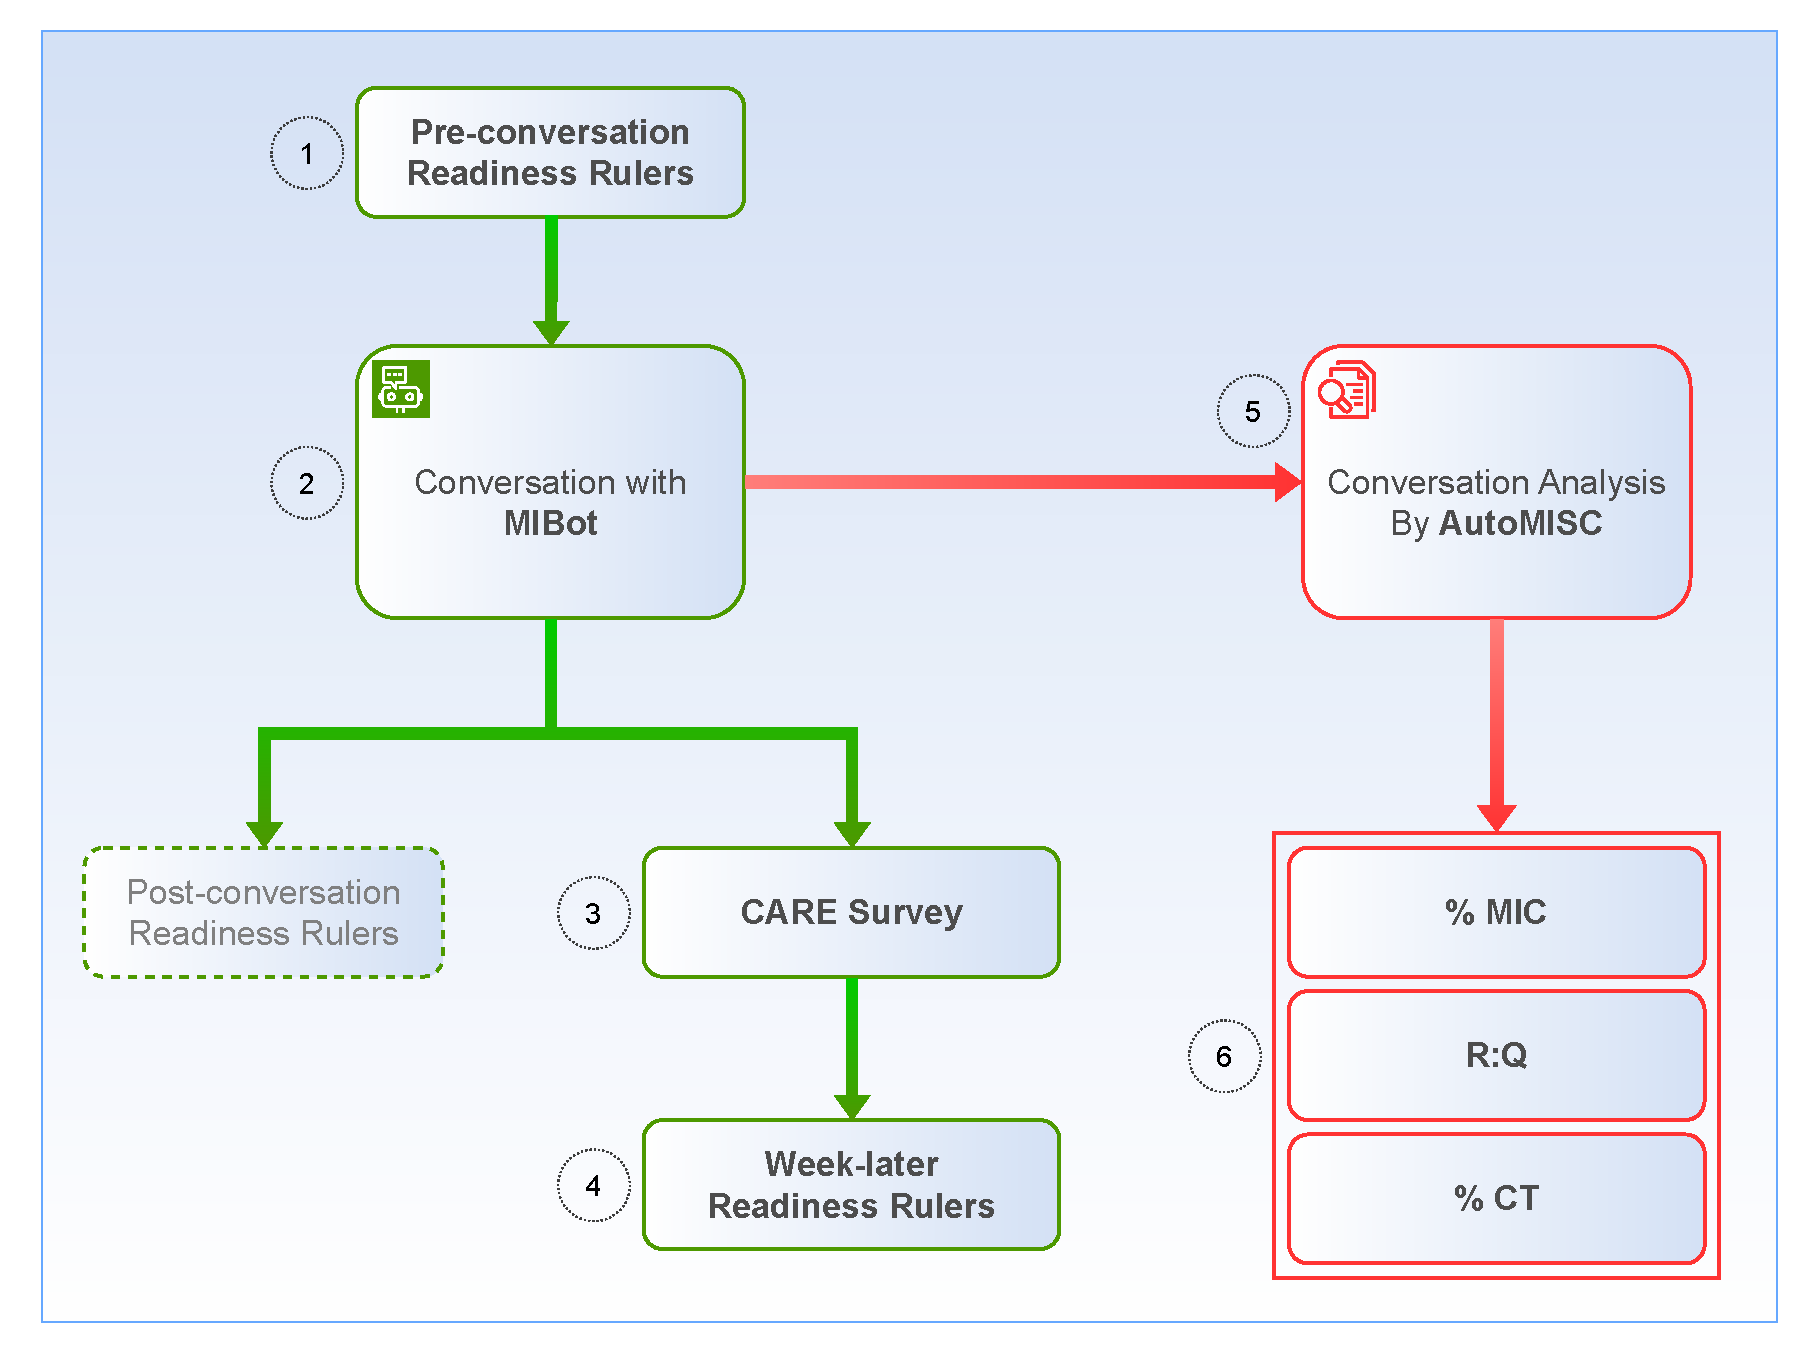
\includegraphics[width=0.9\linewidth]{fig/feasibility_study_flow.pdf}
    \caption[Feasibility Study Protocol Overview]{Overview of the feasibility study protocol, illustrating the four main phases: pre-conversation surveys, a single text-based conversation with MIBot, immediate post-conversation surveys, and a one-week follow-up survey.}
    \label{fig:study-flow}
\end{figure}

The full \margindex[Feasibility Study]{study procedure}study procedure comprised four major phases: (1) \margindex[Feasibility Study, Procedure]{pre-conversation surveys}[Pre-Surveys]pre-conversation surveys; (2) a single text-based conversation with MIBot; (3) \margindex[Feasibility Study, Procedure]{post-conversation surveys}[Post-Surveys]immediate post-conversation surveys; and (4) a \margindex[Feasibility Study, Procedure]{one-week follow-up}[Follow-Up]one-week follow-up survey. Figure~\ref{fig:study-flow} illustrates the progression.



\paragraph{Phase 1: Pre-Conversation Surveys:}
Before interaction with MIBot, participants completed:
\begin{enumerate}
    \item \textbf{\margindex[Feasibility Study, Surveys]{heaviness of smoking index (HSI)}[HSI]Heaviness of Smoking Index (HSI)}~\citep{heatherton1989measuring} survey, which assesses nicotine dependence via two questions:
        \begin{enumerate}
            \item number of cigarettes smoked per day (scored 0-3), and
            \item time to first cigarette after waking (scored 0-3).
        \end{enumerate}
    The HSI score is the sum of these two items, and ranges from 0 to 6, with higher scores indicating greater nicotine dependence.
    \item \textbf{Quit Attempts in the Past Week}: number of conscious attempts to abstain from smoking for at least 24 hours during the preceding seven days.
    \item \textbf{Readiness Ruler}: three questions measuring self-reported ratings of importance, confidence, and readiness to quit on 0–10 scales (Section~\ref{subsec:readiness-ruler}).
\end{enumerate}

\paragraph{Phase 2: Conversation with MIBot:}
Participants engaged in a single MI-style conversation via a web-based text interface.

\paragraph{Phase 3: Post-Conversation Surveys:}
Immediately after the conversation, participants repeated the Readiness Ruler, completed the CARE empathy scale (Section~\ref{subsec:care}), and provided qualitative feedback on the chatbot's performance.

\paragraph{Phase 4: One-Week Follow-Up:}
Seven days later, participants were invited via Prolific to complete a follow-up survey. This included a third administration of the Readiness Ruler and questions about quit attempts and changes in smoking behaviour over the past week.

\subsection{Survey Instruments}
\label{subsec:survey-instruments}

The goal of the work is to move ambivalent smokers towards the decision to quit. We employed the following metrics to measure outcomes from the interaction. In addition to the primary outcome measures, we also recorded other survey instruments to get a holistic picture of the chatbot's effectiveness.

\subsubsection{1. Readiness Ruler}
\label{subsec:readiness-ruler}
The Readiness Ruler~\citep{rollnick1992development} is a validated tool for assessing motivational state across three dimensions:
\begin{itemize}
    \item \textbf{Importance:} ``How important is it to you right now to stop smoking?''
    \item \textbf{Confidence:} ``How confident are you that you would succeed at stopping smoking if you started now?''
    \item \textbf{Readiness:} ``How ready are you to start making a change at stopping smoking right now?''
\end{itemize}
Responses were recorded on an 11-point scale (0 = ``not at all'', 10 = ``extremely''). The week-later change in \emph{confidence} from the pre-conversation value was used as the primary metric for the chatbot's effectiveness, as this is the most predictive
of downstream quitting success~\cite{Gwaltney2009-wj,Abar2013}.

\subsubsection{2. CARE Measure}
\label{subsec:care}
The \margindex[Feasibility Study, Surveys]{care measure}[CARE]Consultation and Relational Empathy (CARE) measure~\citep{mercer2004consultation,bikker2015measuring} assesses perceived empathy in clinical encounters. Ten items evaluate the counsellor's ability to make the participant feel at ease, listen actively, appreciate the participant as a whole person, and collaborate on problem-solving. Each question is rated on a 0-5 scale, with a total score range of 0-50.

\subsubsection{3. Qualitative Feedback}
Three open-ended questions solicited \margindex[Feasibility Study, Surveys]{qualitative feedback}subjective impressions:
\begin{enumerate}
    \item ``What are three words that you would use to describe the chatbot?''
    \item ``What would you change about the conversation?''
    \item ``Did the conversation help you realize anything about your smoking behaviour? Why or why not?''
\end{enumerate}
These responses can inform future prompt refinements and provide contextual data for interpreting quantitative outcomes.

\subsubsection{4. Follow-Up Quit Attempt Survey}
At one week, participants reported whether they had made any quit attempts in the preceding seven days, the number of attempts, and whether any changes in smoking habits had occurred. This included partial changes such as a reduction in cigarettes per day.

\subsection{Automated Conversation Analysis}
\label{subsec:automisc}
In addition to participant-reported outcomes, conversations were analyzed for MI adherence and elicitation of motivational language using \textit{AutoMISC}, an automated implementation of the Motivational Interviewing Skill Code v2.5~\citep{Houck2010}. The AutoMISC system was primarily developed by Soliman, as described in his thesis [CITE\_THESIS], with further validation in~\cite{ali2025automated}. For this project, we utilized the existing AutoMISC system and contributed to the work described in~\cite{mahmood-etal-2025-fully}. The analysis pipeline first segments each conversational volley into individual utterances. Then, it classifies counsellor utterances as MI-Consistent, MI-Inconsistent, Reflection, Question, or Other. Similarly, it classifies each client utterance as exhibiting Change Talk, Sustain Talk, or Neutral. Finally, it computes the following: \%~MI-Consistent Responses (\%MIC), Reflection-to-Question Ratio (R:Q), \%~Client Change Talk (\%CT). AutoMISC was validated against human coders, including two MI-expert clinicians \cite{mahmood-etal-2025-fully}.


Readiness rulers (especially the week-later change in \emph{confidence}), CARE, and AutoMISC summary metrics together provide a holistic view of the MIBot intervention, assessing its effectiveness, perceived empathy, safety, and adherence to MI principles. In the next chapter, we report the results from our human feasibility study on these metrics.
